\documentclass[11pt]{article}
\usepackage{textcomp,bbding,subfig}
\usepackage{float,amssymb,amsmath,amsfonts,bm}
\usepackage{graphicx,cite}
\usepackage[]{natbib}
\def\style{apa}
\usepackage[usenames,pdftex,dvips]{color,xcolor}
\usepackage{multirow,tabulary,colortbl,array}
\usepackage[normalem]{ulem}
\usepackage[colorlinks,bookmarksopen,bookmarksnumbered,citecolor=blue,urlcolor=blue]{hyperref}
\usepackage{moreverb,setspace}
%
% Text layout
\topmargin -1.5cm
\oddsidemargin 0.0cm
\evensidemargin 0.0cm
\textwidth 16.5cm
\textheight 23.5cm     
%
% Remove brackets from numbering in List of References
% \makeatletter \renewcommand\@biblabel[1]{} \makeatother
\makeatletter
\renewcommand{\@biblabel}[1]{\quad#1.}
\makeatother
%
% aliasis
% FreeSurfer from Havord Unv.
\newcommand{\FS}{\href{http://surfer.nmr.mgh.harvard.edu}{\textbf{FreeSurfer}}} 
\newcommand{\bs}{\boldsymbol}
% xiaoran's edit
\newcommand{\xadd}[1]{\textcolor{blue}{#1}}
\newcommand{\xdel}[1]{\textcolor{red}{\sout{#1}}}
\newcommand{\xrpl}[2]{\xdel{#1}\xadd{#2}}
\newcommand{\xacc}[1]{\textcolor{ForestGreen}{#1}}
%
% encoders
% vector or matrix
\newcommand{\vecEC}[1]{\boldsymbol{#1}}
%
% decoders
\newcommand{\vecDC}[1]{\boldsymbol{\tilde{#1}}} 
%
\newcommand{\xVO}{\boldsymbol{x}}         % the x vector, original
\newcommand{\xVR}{\boldsymbol{\tilde{x}}} % the x vector, recovered
\newcommand{\xSO}{x}                      % the x scaler, original
\newcommand{\xSR}{\tilde{x}}              % the x scaler, recovered
%
% the eta vector
\newcommand{\etaEC}{\vecEC{\eta}}                % generic encoder
\newcommand{\etaEi}{\WEC_i^{d_{i+1} \times d_i}} % encoder layer i
\newcommand{\etaDC}{\vecDC{\eta}}                % generic decoder
\newcommand{\etaDi}{\WDC_i^{d_i \times d_{i+1}}} % decoder layer i
%
% the W matrix
\newcommand{\WEC}{\vecEC{W}}                   % generic encoder
\newcommand{\WEi}{\WEC_i^{d_{i+1} \times d_i}} % encoder layer i
\newcommand{\WEI}[3]{\WEC_{#1}^{d_{#2} \times d_{#3}}} % decoder layer #i
\newcommand{\WEIt}[3]{\WEC_{#1}^{d_{#2} \times d_{#3}\prime}} % decoder layer #i, transposed
\newcommand{\WDC}{\vecDC{W}}                   % generic decoder
\newcommand{\WDi}{\WDC_i^{d_i \times d_{i+1}}} % decoder layer #i
\newcommand{\WDI}[3]{\WDC_{#1}^{d_{#2} \times d_{#3}}} % decoder layer #i
\newcommand{\WDIt}[3]{\WDC_{#1}^{d_{#2} \times d_{#3}\prime}} % decoder layer #i

% the w vector
\newcommand{\wEC}{\vecEC{w}}    % generic encoder
\newcommand{\wEI}[2]{{\wEC_{#1}^{1 \times d_{#2}}}}
\newcommand{\wDC}{\vecDC{w}}    % generic decoder
\newcommand{\wDI}[2]{{\wDC_{#1}^{1 \times d_{#2}}}}
\newcommand{\wDIt}[2]{{\wDC_{#1}^{1 \times d_{#2}\prime}}}

% the b vector
\newcommand{\bEC}{\vecEC{b}}    % generic encoder
\newcommand{\bEi}{\bEC_i^{d_i}} % encoder layer i
\newcommand{\bEI}[2]{\bEC_{#1}^{d_{#2}}} % encoder layer i
\newcommand{\bDC}{\vecDC{b}}    % generic decoder
\newcommand{\bDi}{\bDC_i^{d_i}} % encoder layer i
\newcommand{\bDI}[2]{\bDC_{#1}^{d_{#2}}} % encoder layer i

% the x vector
\newcommand{\xEC}{\vecEC{x}}
\newcommand{\xDC}{\vecDC{x}}
% the X matrix
\newcommand{\XEC}{\vecEC{X}}
\newcommand{\XDC}{\vecDC{X}}
%
% the y_hat vector
\newcommand{\yHT}{\boldsymbol{\hat{y}}}
\newcommand{\YHT}{\boldsymbol{\hat{Y}}}
\newcommand{\hHT}{\boldsymbol{\hat{h}}}
\newcommand{\HHT}{\boldsymbol{\hat{H}}}
%
% the z vector
\newcommand{\zEC}{\vecEC{z}}
\newcommand{\zDC}{\vecDC{z}}
%
% I/O for decoder layer
\newcommand{\iDi}{\zDC_{i+1}^{d_{i+1}}}
\newcommand{\zEI}[2]{\zEC_{#1}^{d_{#2}}}
\newcommand{\zEIt}[2]{\zEC_{#1}^{d_{#2}\prime}}
\newcommand{\oDi}{\zDC_i^{d_i}}
\newcommand{\zDI}[2]{\zDC_{#1}^{d_{#2}}}
\newcommand{\zDIt}[2]{\zDC_{#1}^{d_{#2}\prime}}
%
% the vector of ones
\newcommand{\one}{\boldsymbol{1}}
% the diagnal matrix
\newcommand{\I}[1]{\boldsymbol{I}^{#1}}
%
% parameters in the neural network
\newcommand{\Par}{\boldsymbol{\Theta}}
\newcommand{\pEC}{\boldsymbol{\theta}}
\newcommand{\pDC}{\boldsymbol{\tilde{\theta}}}
%
% Loss function in Cross Entropy form
\newcommand{\LCE}[2]{#1\log{#2} + (1-#1)\log{(1-#2)}}
%
% derivative
\newcommand{\DRV}[2]{\frac{d #1}{d #2}}
\newcommand{\DRC}[3]{\DRV{#1}{#2}\DRV{#2}{#3}}
\newcommand{\PDV}[2]{\frac{\partial #1}{\partial #2}}
\newcommand{\PDC}[3]{\PDV{#1}{#2}\PDV{#2}{#3}}
%
% invers logit, aka. sigmoid function
\newcommand{\SGM}[1]{\frac{1}{1+e^{-#1}}}
%
% assign to diagnoral
\newcommand{\diag}[1]{\text{diag} (#1)}

% \pagestyle{headings}

% \author{Xiaoran Tong, Qin Lu} 
\doublespacing
\begin{document}
\title{An Joint Association Analysis Method for Genomic Sequencing and Neuroimaging Data}
\maketitle
\begin{flushleft}
Xiaoran Tong\textsuperscript{1},
Olga Vsevolozhskaya\textsuperscript{2},
Qin Lu\textsuperscript{1*},
\\
\bigskip
\textbf{1} Department of Epidemiology and Biostatistics, Michigan State University, East Lansing, USA
\textbf{2} Department of Biostatistic, University of Kentucky College of Public Health

\vskip 50ex
Correspondence: Qing Lu\\
Department of Epidemiology and Biostatistics\\
College of Human Medicine\\
Michigan State University\\
909 Fee Road\\
East Lansing, MI 48824--1030\\
qlu@msu.edu\\
\end{flushleft}

\clearpage
\begin{abstract}
Despite heightened interest in the genetic basis of human disease, genome-wide studies have explained relatively little of the heritability of most complex traits and variants identified through these studies have small effect sizes. Although it is hard to provide a single answer to the question of where to find missing heritability, researchers are recently leaning towards using genetic risk factors in combination with clinical biomarkers to gain further knowledge on various phases of complex diseases. For instance, it has been suggested that imaging data that characterizes functional brain abnormalities combined with genetic variability may help researchers identify individuals at risk for Alzheimer's disease. However, a joint analysis of imaging and genetic data presents challenges due to high dimensionality and high redundancy of medical data, leading to a significant decrease in statistical power of any association test. In this work, we incorporate imaging profile to empower the genomic association analysis through the use of the similarity U-statistic. To tackle high dimensionality and high redundancy of imaging data, we use machine learning techniques to replace raw image with abstracted higher order features. We demonstrate flexibility and competitive power of our approach gained by replacing raw neuroimage with high order features through extensive simulation studies. Further, we illustrate potential for discovery of our method through a joint analysis of imaging and genetic data from the Alzheimer’s Disease Neuroimaging Initiative (ADNI).
\end{abstract}
\clearpage
\section*{Introduction}
Despite a decade long effort, genome wide association (GWA) analysis has fell short in providing definitive evidence for casual genetic variants for most common human complex diseases. Although a large number of statistically significant common variants were indeed identified by GWA, only a moderate fraction of heritability has been explained by the totality of these findings~\citep{GWA1, GWA2}. The ``rare variant, common disease (RVCD)'' hypothesis was aimed to explain the missing heritability which GWA failed to capture. RVCD states that the missing heritability gap could be attributed to rare variants with moderate to large effect sizes that were not covered by GWA~\citep{RVCD1}. The Next Generation Sequencing (NGS) project, growing in both numbers and scale over the last decade, offered numerous data sources for the analysis of rare variants. However, the stockpiling data also raised a number of methodological challenges. For one, the variants in the NGS profile are much denser than those in a GWA profile, which poses intense computational and multiple testing burden on the traditional per-variant based screening procedures. Also, as the name suggests, the newly detected rare variants have minor allele frequencies (MAF) close to zero. As a consequence, studies with a small or a moderate sample size may have low statistical power due to the lack of genetic heterogeneity in the sample. 

Signal aggregation was proposed as a solution for rare variants' computational issue~\citep{Burden1, UST1, UST2, SKAT, GCTA, Dai:2015, plink1}. With signal aggregation, instead of screening the whole profile one variant at a time, variants are first grouped according to a certain criteria and then all variants in a group are tested together as a single unit. The aggregation can be achieved by either collapsing all grouped variants into a single variant before a statistical test~\citep{Burden1}, or by testing all variants together with a multivariate approach~\citep{UST1, UST2, SKAT, GCTA}. Alternatively, the aggregation can be done after per-variant screening by combining group members' statistics. (e.g., p-values)~\citep{Dai:2015, plink1, zaykin2002truncated}. Grouping and aggregation drastically reduces the number of hypothesis to be tested and improves heterogeneity over any of its member variant. However, the choice of a grouping criteria poses a challenge. The most common choice is to refer to the prior knowledge of biological function, resulting in gene or pathway based grouping (e.g., \cite{vsevolozhskaya2016uncovering}). Alternatively, the grouping can be based on physical distance such as grouping by every few thousand nucleotide base-pairs or by a threshold of linkage disequilibrium (LD)~(e.g., \cite{plink1}).

Besides rare variants, an important factor that has been argued to contribute to the unsatisfactory performance of GWA is the fact that complex diseases have intrinsically weak genetic effects due to a large ``black box'' between the upstream genomic variants and the downstream health outcomes. Therefore, it is desirable to probe this ``black box'' by incorporating intermediate biological profiles, with the hope that the added information will increase chances of detecting stronger associations, especially when the biomarkers in these new profiles are mediating the genetic casual effect on the disease. 

In this paper, we propose a new method that incorporates neuroimaging information into the genomic association analyses and augments statistical power with these ``added data.'' The cortex structure captured by imaging devices is a powerful predictor of a neurological disorder and should be jointly analyzed with a genomic profile. Techniques similar to GAW have been developed for imaging data, given a proper definition of an ``image variant'' and its value. Taking the structured magnetic resonance imaging (MRI) as an example, it is natural to view a voxel in a pile of slices as a ``variant'' and the normalized brightness of that voxel as its value. Alternatively, if a three-dimensional (3D) cortex spanned by hundreds of thousands vertices is used, every vertex can be seen as an image variant, while the 3D coordinates of that vertex, the thickness and the curvature of cortex around that vertex, can be seen as its value. These definitions gave rise to a voxel-wise analysis~\citep{VWA1, VWA2, VWA3, VWA4} or to a vertex-wise analysis~\citep{FS:Anl1, FS:Anl2}, both abbreviated as ``VWA'' for short. With ideas similar to GWA, VWA applies a per-voxel or per-vertex screening procedure to detect significant loci in the brain. On the one hand, this imaging per-unit analysis is less troublesome than that of a NGS profile because there are no ``rare'' variants, since imaging data values (e.g., brightness of a voxel or thickness at a vertex) are continuous. On the other hand, imaging profiles are also high dimensional with a large number of voxels or vertices, raising computational and multiple testing issues quiet similar to those encountered with NGS data. Yet again, grouping and aggregation techniques that work with NGS analysis may also help in studies involving imaging data. For example, grouping can be achieved by partitioning a 3D cortex surface into well defined functional anatomical regions (e.g., 68 symmetrical regions, 34 per hemisphere) and considering all vertices in a regions as a single unit for the analysis. Regions so defined will contain from a few hundred to more than ten thousand vertices -- a much larger value than a typical number of variants in a gene. However, due to their proximity, vertices exhibit high correlation and redundancy (because they represent a tightly connected brain tissue) and the number of ``independent'' vertices can be much smaller. One approach to reduce the number of correlated vertices that is recently gaining enormous popularity in computer science is the unsupervised training of deep artificial neural networks (ANN) capable of abstracting high order features from a raw image. The high order features have lower dimension but higher signal-to-noise ratio than the image itself~\citep{DL:Intro1, DL:SDA1, DL:Intro2}. Additionally, an unsupervised ANN is capable of cumulatively refining itself with incoming new knowledge. In other words, as long as the future 3D cortex data shares compatible format with the one currently in use, the deep ANN trained today can be re-calibrated to extract more informative features from future data.

In this study, we propose to use the stacked autoencoder (SA), a type of unsupervised deep ANN trained with the maximum likelihood based, gradient guided numerical optimization techniques, to reduce the dimensionality of imaging data (\cite{DL:SDA1, DL:Intro2}). Then, we adopt a similarity measure based on a U-statistic \citep{UST1, UST2} to jointly analyze collapsed genomic and imaging profiles. We show that our newly proposed joint analysis is robust against various types of model misspecification and is faster than the main stream algorithms that currently support multiple aggregated high dimensional components such as SKAT~\citep{SKAT} or GCTA~\citep{GCTA}. Additionally, we show improvement in statistical power if high order features abstracted by the trained SA are used instead of the raw image profile.

The rest of this paper is organized as follows. In the Methods sections, we detail unsupervised training of stacked autoencoder and the resulting abstraction of high order features from a 3D cortex image, followed by the joint analysis of genomic and imaging profiles (either with the raw cortex data or with the higher order features) via a U-statistics. Further, through simulation studies, we report performance gained by adopting the joint test, the grouping and aggregation strategy on imaging profile, and the replacement of raw imaging with high order features.  Finally, we showcase our approach by jointly analyzing case-control imaging and genetic data from the Alzheimer’s Disease Neuroimaging Initiative (ADNI)~\citep{ADNI05, ADNI10}.

\section*{Methods}

\subsection*{Processing Imaging Profile with Stacked Autoencoder}

A stacked autoencoder (SA) is an artificial neural network (ANN) mimicking visual processing that abstracts high order features from a raw image. These high order features can typically be more relevant to decision making than the original per-pixel color values of an image. For example, knowing the exact thickness and curvature of every point in the 3D cortex image may be less helpful for a physician in diagnosis of a neurodegenerative disorder than being able to recognize the general location, size and shape of the laceration sites in the same cortex image. Thus, by learning high order features with the SA algorithm, 
while disregarding trivial and redundant details, we expect to achieve a power boost in a subsequent association analysis, given that these features are appropriate for replacing the unprocessed imaging profile.

A stacked autoencoder is comprised of two or more encoders stacked on top of each other. An encoder is an information preserving transformation that produces a more concise output than the input. In other words, an SA is a linear recombination of the input entries followed by an entry-wise non-linear transformation. An $i$th encoder in a stack of $M$ layers can be written as:
\begin{equation} \label{eq:AE}
  \zEC_i^{d_i} = \boldsymbol{s}(\WEI{i}{i}{i-1} \zEI{i-1}{i-1} + \bEI{i}{i}), \quad i = 1, \ldots, M,
\end{equation}
where $\zEI{i}{i}$ is the $i$th encoder's $d_i$ dimensional output, and $\zEI{i-1}{i-1}$ is $d_{i-1}$ dimensional input, which, in turn, is also an output from the encoder down below, (i.e., $(i-1)$th in the stack). A linear recombination of the input is achieved by a $(d_{i-1} \times d_i)$ weight matrix $\WEI{i}{i}{i-i}$ and a $(d_i\times 1)$ offset vector $\bEI{i}{i}$. The function $\boldsymbol{s}(\cdot)$ denotes an aforementioned entry-wise non-linear transformation. A popular choice for $\boldsymbol{s}(\cdot)$ includes the ``$S$''-shaped inverse logit function that can mimic neuron activation~\citep{SGM1, NNE90}. Finally, being an encoder demands the output size $d_i$ to be smaller than the input size $d_{i-1}$, which in turn ensures that dimension reduction and high order feature abstraction actually happens.

Once an encoder is defined, one can assemble a stack of $M$ encoders that accepts size $P$ input vector, $\xEC^P$, and produces size $Q<P$ high order feature vector, $\hHT^Q$, by recursively wiring the output of an encoder to the one above it, and ensuring that the input dimensionality at the bottom, $d_0$, equals to $P$, and the output dimensionality on the top, $d_M$, equals to $Q$. Mathematically, the encoder stack can be written as:
\begin{equation} \label{eq:SE}
  \begin{split}
    \hHT^Q &= \zEI{M}{M} \\
    \zEI{M  }{M  } &= s(\WEI{M  }{M  }{M-1} \zEI{M-1}{M-1} + \bEI{M  }{M  }) \\
    \zEI{M-1}{M-1} &= s(\WEI{M-1}{M-1}{M-2} \zEI{M-2}{M-2} + \bEI{M-1}{M-1}) \\
    & \quad \quad \quad \quad \vdots \\
    \zEI{i  }{i  } &= s(\WEI{i  }{i  }{i-1} \zEI{i-1}{i-1} + \bEI{i  }{i  }) \\
    & \quad \quad \quad \quad \vdots \\
    \zEI{2  }{2  } &= s(\WEI{2  }{2  }{1  } \zEI{1  }{1  } + \bEI{2  }{2  }) \\
    \zEI{1  }{1  } &= s(\WEI{1  }{1  }{0  } \zEI{0  }{0  } + \bEI{1  }{1  }) \\
    \zEI{0  }{0  } &= \xEC^P.
  \end{split}
\end{equation}
Here, the $P$-dimensional input $\xEC^P$ can be viewed as the output of the non-existing $0$th encoder. By restricting $P = d_0 > d_1 > d_2 > \cdots > d_{M-1} > d_M = Q$, the encoder stack abstracts $Q$ dimensional high order features from the $P$ dimensional raw profile. To ensure that the output is a concise preservation of the input, the parameters of the stack, that is, the weights and the offsets, $\{\WEC_1, \bEC_1, \WEC_2, \bEC_2, \dots, \WEC_M, \bEC_M\}$, must be tuned to represent the body of knowledge that generated $\xEC^P$, which in our case is the knowledge of human cortex. To do so, we assemble a stacked encoder counterpart, i.e., a stacked decoder that starts with higher order features and outputs the entire image. The stacked decoders exactly mirror the topology of the initial encoders:
\begin{equation} \label{eq:SD}
  \begin{split}
    \xDC^P &= \zDI{0}{0} \\
    \zDI{0  }{0  } &= s(\WDI{1  }{0  }{1  } \zDI{1  }{1  } + \bDI{1  }{0  }) \\
    \zDI{1  }{1  } &= s(\WDI{2  }{1  }{2  } \zDI{2  }{2  } + \bDI{2  }{1  }) \\
    & \quad \quad \quad \quad \vdots \\
    \zDI{i-1}{i-1} &= s(\WDI{i  }{i-1}{i  } \zDI{i  }{i  } + \bDI{i  }{i-1}) \\
    & \quad \quad \quad \quad \vdots \\
    \zDI{M-2}{M-2} &= s(\WDI{M-1}{M-2}{M-1} \zDI{M-1}{M-1} + \bDI{M-1}{M-2}) \\
    \zDI{M-1}{M-1} &= s(\WDI{M  }{M-1}{M  } \zDI{M  }{M  } + \bDI{M  }{M-1}). \\
  \end{split}
\end{equation}
The weights of the stacked decoders also mirror the weights of the stacked encoders:
\begin{align}
  \WDI{M-i}{M-i-1}{M-i} \equiv {(\WEI{M-i}{M-i}{M-i-1})}^\prime, \quad (i=0, \dots, M),
\end{align}
However, the offsets in the decoders, $\bDI{M-i}{M-i-1}, (i=0, \dots, M)$, are allowed to be flexible \citep{DL:SDA1}. This approach to tune the parameters of the stack is quiet instinctive since decoding is the opposite of encoding. From the bottom to the top, this stack of decoders gradually restores details back to the abstracted state $\zDI{M}{M}$ and eventually presents a reconstructed input $\xDC^P$ on its top.

One can combine Eq.~(\ref{eq:SE}) and (\ref{eq:SD}) by setting $\zDI{M}{M} = \hHT^Q$,
\begin{equation} \label{eq:SA}
  \begin{split}
    \xDC^P &= \zDI{0}{0} \\
    \zDI{0  }{0  } &= s(\WDI{1  }{0  }{1  } \zDI{1  }{1  } + \bDI{1}{0  }) \\
    & \quad \quad \quad \quad \vdots \\
    \zDI{M-1}{M-1} &= s(\WDI{M  }{M-1}{M  } \zDI{M  }{M  } + \bDI{M}{M-1}) \\
    \zDI{M  }{M  } &= \hHT^Q = \zEI{M}{M} \\
    \zEI{M  }{M  } &= s(\WEI{M  }{M  }{M-1} \zEI{M-1}{M-1} + \bEI{M}{M  }) \\
    & \quad \quad \quad \quad \vdots \\
    \zEI{1  }{1  } &= s(\WEI{1  }{1  }{0  } \zEI{0  }{0  } + \bEI{1}{1  }) \\
    \zEI{0  }{0  } &= \xEC^P,
  \end{split}
\end{equation}
which creates a stacked autoencoder \citep{DL:SDA1}. The aforementioned weights and offsets in the encoder stack (the lower half of the SA), alongside with $M$ extra offsets in the decoder stack (the upper half of the SA), constitute the parameters to be calibrated in order to make the encoder stack to be a close represent of the process that generated $\xEC^P$. The calibration is done by minimize the discrepancy between the reconstructed input $\xDC^P$ and the true input $\xEC^P$. The rationale is that if the compact code $\hHT$ presented by the encoder stack truly captures the major features of $\xEC^P$, the restored input, $\xDC^P$, should be nearly identical to the original one, except some trivial details. Tuning the encoder stack is equivalent to solving the following optimization problem:
\begin{equation} \label{eq:CE}
  \begin{split}
    \Par^* = \min_{\Par} \sum_{k=1}^N{d(\xDC_k^P, \xEC_k^P)}, \quad \Par = \cup_{i=1}^M \{\WEC_i, \bEC_i, \bDC_i\},
  \end{split}
\end{equation}
where $k$ indices $N$ training samples. The objective function, $d$, measures the disagreement between the reconstructed and the original input. A popular form of $d$ is a cross-entropy:
\begin{align} \label{eq:CE}
  d(\xDC_k^P, \xEC_k^P) = \sum_{j=1}^P[{x_{j,k}\log{\tilde{x}_{j,k}} + (1 - x_{j,k})\log{(1 - \tilde{x}_{j,k})}}],
\end{align}
where $j$ indices $P$ entries of the input. 

Optimization of a large number of parameters (cardinality of $|\Par| = \sum_{i=1}^M{d_i d_{i-1} + d_i + d_{i-1}}$) is achieved by stochastic gradient descent (SGD)~\citep{SGD1, SGD2}, which is also called the back propagation (BP) algorithm by neural network literature concerning computations of high dimensional gradients~\citep{BP1, BP2, BP3}. For practical implementation of SGD and BP algorithms, a Python~\citep{python1} library Theano~\citep{Theano1} can be used.

Optimization of deep neural networks, (i.e., an SA with many layers of encoders and decoders) is challenging due to the increased prevalence of local minimum site in the error terrain and relatively slow convergence rates. To address these issues, we follow the ``deep learning'' trend, which is recently becoming increasingly popular and by which a layer-wise greedy pre-training procedure is applied prior to fine-tuning the entire network~\citep{DL:DBN1, DL:SDA1}. To do so, the output of the $i$th encoder, $\zEC_i$, is disconnected from the encoder above it and rewired to its decoder's counterpart, immediately forming a single layered autoencoder, which is then calibrated by minimizing the intermediate reconstruction loss $d(\zEC_{i-1}, \zDC_{i-1})$. That is,
\begin{equation}\label{eq:Greedy}
  \begin{split}
    \zDC_{i-1} &= s(\WDC_i \zDC_i + \bDC_i) \\
    \zDC_{i  } &= \hHT_i = \zEC_i \quad \qquad \qquad \qquad (i = 0 \dots M) \\
    \zEC_{i  } &= s(\WEC_i\zEC_{i-1} + \bEC_i). \\
    \pEC_i^* &= \min_{\pEC_i}{d(\zEC_{i-1}, \zDC_{i-1})}, \qquad \pEC_i = \{\WEC_i, \bEC_i, \bDC_i\},
  \end{split}
\end{equation}
This optimization problem is much easier than the one in Eq.~(\ref{eq:SA}) due to a smaller number of parameters ($|\pEC_i|=d_i d_{i-1} + d_i + d_{i-1}$). Then, after all $M$ single-layer autoencoders are pre-trained, the encoders and decoders are wired back to Eq.~(\ref{eq:SA}) and fine-tuned together, resulting in faster convergence and less likely chances of ``going down the wrong pit'' in the terrain of $d(\xDC_k^P, \xEC_k^P)$.

For the current project, we let each encoder halve its input (i.e., $d_i = d_{i-1}/2$). Then, for each cortex region we form an $M=4$ layered SA, achieving a $16$ fold dimension reduction. Further, we use higher order features extracted by the SA in place of the raw imaging profile in the subsequent statistical analysis.


\subsection*{Joint Test with the U-statistic}
\newcommand{\vg}{\boldsymbol{g}}
\newcommand{\vv}{\boldsymbol{v}}
We use a similarity measure based on the U-statistic~\citep{UST1, UST2} to jointly test for an association between a phenotype of interest (either quantitative or qualitative) and genomic and imaging profiles combined. To derive the statistic, three kernel functions measuring pairwise similarity are chosen for each profile. The measurement, $f(\cdot)$, can be flexible to suit specific characteristics of a profile (e.g.\ bounded or not, continuous or discrete), as long as $f$ is symmetric and has a finite second moment (i.e., $f(x_i,x_j) \equiv f(x_j,x_i)$ and $E(f^2(x_i, x_j))<\infty$).

For genomic profile coded by minor allele count (0, 1 or 2), we use the Identical By State (IBS) kernel:
\label{eq:wSG}
\[ f_G(\vg_{i.}, \vg_{j.}) = \frac{\sum_{m=1}^{|\bs{G}|}{w_m(2 - |g_{im} - g_{jm}|)}} {2\sum_{m=1}^{|\bs{G}|}{w_m}}, \]
where $(i,j)$ indices a pair of observations for subjects $i$ and $j$, $m$ indices a genomic variant (i.e., a SNP) in the testing unit (e.g., a gene $\bs{G}$), and $w_m$ is the weight assigned to the $m$th variant according to \textit{a prior} hypothesis. For example, weights can be assigned based on the allele frequency ($AF$) as $w_m=\sqrt{AF(g_{.m})[1-AF(g_{.m})]}$ to emphasize the effect of rare variants.

The imaging profile can either be a raw 3D cortical surface vertices or the high order features abstracted from them by an SA. For both, we can use the Gaussian kernel, which is well suited for continuous values,
\label{eq:wSV}
\[ f_V(\vv_{i.},\vv_{j.}) = \exp{\left[-\frac{1}{|\bs{V}|} \sum_{m=1}^{|\bs{V}|}{(v_{im}-v_{jm})^2} \right]}. \]
Here, $m$ indices a variant  (e.g., a vertex) in a cortex region $\bs{V}$ (e.g., superior-temporal, entorhinal, ect.). 

Then, the entry-wise product of genomic and imaging kernels forms the joint predictor kernel $\bs{K}^J$ as follows:
\[ K_{ij}^J = f_G(\vg_{i.}, \vg_{j.}) f_V(\vv_{i.}, \vv_{j.}).\]
Further, the entries in the predictor kernel $\bs{K}^J$ are centered by subtracting two marginal means (for both subjects $i$ and $j$) and by adding the overall mean~\citep{UST2}, so that:
\begin{align*}
  \tilde{K}_{ij}^J = K_{ij}^J -\frac{1}{N} \sum_{k=1}^N{K_{ik}^J}-\frac{1}{N}\sum_{l=1}^N{K_{lj}^J} + \frac{1}{N^2} \sum_{k=1}^{N} \sum_{l=1}^{N} {K_{lk}^J},
\end{align*}
where $N$ is the number of subjects. 

Lastly, for a phenotype profile generated by an unknown distribution, we first normalized it by the rank normal quantile transformation:
\[ q_i = \frac{\Phi^{-1}[\text{rank}(y_i - 0.5)]}{N}, \]
where $y_i$ is the phenotypic measure for the $ith$ subject. Next, we project the transformed phenotype $\bs{q}$ onto the space spaned by $P$ covariate $\bs{X}=[\bs{1}, \bs{x}_1, \dots, \bs{x}_P]$ through a linear regression. The residual terms of this regression are then used to build a similarity measure for phenotypes via the cross-product kernel~\citep{UST1}:
\[ \hat{H}_{ij} = \tilde{f}_Y(q_i, q_j) = \frac{(q_i - \hat{q}_i)(q_j - \hat{q}_j)}{(\bs{q}-\bs{\hat{q}})^\prime(\bs{q}-\bs{\hat{q}})/(N-P-1)}. \]
where $\hat{\bs{q}} = \bs{X}(\bs{X}^\prime\bs{X})^{-1}\bs{X}^\prime \bs{q}$ is the predicted mean phenotype vector, given covariates $\bs{X}$. After this projection, phenotype similarities are already centered and one can use $\hat{\bs{H}}$. as the response kernel. To make the test statistics more robust against residual confounding, \cite{HWU1} also suggested to project the similarity kernel among predictors ${\bs\tilde{K}}^J$ onto the covariates space and use the resulting residuals as a new measure orthogonal to $\bs{X}$,
\[ \bs{\hat{K}}^J = (\bs{I} - \bs{X}(\bs{X}^\prime\bs{X})^{-1}\bs{X}^\prime) \bs{\tilde{K}}^J (\bs{I} - \bs{X}(\bs{X}^\prime\bs{X})^{-1}\bs{X}^\prime). \]
Then, the joint similarity U-statistic, $U_J$, can be defined as the mean of entry-wise products between the response kernel $\bs{H}$ and the predictor kernel $\bs{K}^J$, excluding self-pairs $i=j$, as:
\[ U_J = \frac{2}{N(N-1)} \sum_{1 \leq i < j \leq N}^{} \hat{H}_{ij} \hat{K}_{ij}^J \]
Under the null hypothesis of no association between any of the profiles, $U_J$ should be close to $0$ since all centered kernel measurements should have zero means. Conversely, significant deviations of $U_J$ from $0$ will imply an association. Formally, under $H_0$,  $U_J$ follows a weighted mixture of the $\chi_1^2$ distributions~\citep{UST1},
\[ U_J \sim \frac{1}{N} \sum_{m=1}^\infty{\alpha_m \sum_{l=1}^N{\hat{\lambda}_l (\chi^2_{1,ml} - 1)} }, \]
where $\alpha_m$ is an eigenvalue of response similarity kernel function $f_Y(\cdot, \cdot)$, approximated by $\bs{H}$, and $\hat{\lambda}_l$ is an eigenvalue of predictor kernel $\bs{\hat{K}}\textcolor{red}{^J}$. When a cross-product kernel is used for $f_Y$, $\alpha_1 = 1$, and $\alpha_m = 0, (m > 1)$, and the mixture can be simplified as \citep{UST1},
\[ U_J \sim \frac{1}{N} \sum_{l=1}^\infty{\hat{\lambda}_l \chi^2_{1,l}}. \]
A p-value based on this chi-squared mixture can be approximated by the Davis method~\citep{davies80}.

Alternatively, two simpler tests can be performed by dropping either the imaging or the genomic kernels. That is,
\[ K_{ij}^G = f_G(\vg_{i.}, \vg_{j.}), \quad \text{or}\quad K_{ij}^V = f_V(\vv_{i.}, \vv_{j.}), \]
which are subsequently center and projected onto $\bs{X}$ just as in the case of $\bs{K}^J$. The simplified test based on the:
\[ U_G = \frac{2}{N(N-1)} \sum_{1 \leq i < j \leq N}^{} \hat{H}_{ij} \hat{K}_{ij}^G \]
will test for an association between a phenotype and the genomic profile. And,
\[ U_V = \frac{2}{N(N-1)} \sum_{1 \leq i < j \leq N}^{} \hat{H}_{ij} \hat{K}_{ij}^V \]
will test for an association between a phenotype and the imaging profile. These two tests are more specific and correspond to more parsimonious models. However, they also run the risk of model misspecification, a sensitivity to which will be explored in a simulation study.

The imaging similarity measure described just above aggregates all signals of all vertices in one testing unit $\bs{V}$. For comparison purposes, in our simulation studies, we also implemented a per-vertex analysis, that is, the vertex-wise analysis (VWA). Briefly speaking, for the per-vertex analysis, we first smoothed the imaging profile with a Gaussian filter to reduce noise and grind away trivial details in a 3D cortex. Next, for each one of the $|\bs{V}|$ vertices, we performed a test based on the $U_J$ or $U_V$ statistic, and the resulting $|\bs{V}|$ p-values were corrected against multiple testing according to the false discovery rate (FDR) criteria \citep{FDR}. If at least one FDR corrected p-value was below the $0.05$ threshold, the entire testing unit of $|\bs{V}|$ vertices was declared statistically significant.

\section*{Result}
\subsection*{Simulation Study Setup}
To mimic the real sequencing and imaging data structure, we based our simulations on observations from 806 participants of the Alzheimer's Disease Neuroimaging Initiative (ADNI) \citep{ADNI05, ADNI10} with information over both NGS and MRI profiles. The 3D cortex was re-built from MRI data using Freesurfer software~\citep{FS:Intro}. In each simulation iteration, we picked a gene, $\bs{G}$, and a cortex region of 512 vertices, $\bs{V}$, (roughly a circle of 28mm in diameter), and assigned an effect size to 5\% of the genomic and imaging variants. Non-zero effect sizes were drawn from a standard normal distribution. Then, we generated two phenotypes solely based on a genomic or an imaging effect, $\bs{Y}_G$ and $\bs{Y}_V$, respectively; added them up to get an additive effect $\bs{Y}_A$; obtained their entry-wise product for an interaction effect $\bs{Y}_I$. More formally, 
\begin{equation}\label{eq:SM1}
  \begin{split}
    \bs{Y}_G &= \bs{\beta}_G \bs{X}_G + \bs{\epsilon}_G, \quad \beta_{.G} \sim N(0,1) \times \text{Bernoulli}(0.05), \\
    \bs{Y}_V &= \bs{\beta}_V \bs{X}_V + \bs{\epsilon}_V, \quad \beta_{.V} \sim N(0,1) \times \text{Bernoulli}(0.05), \\
    \bs{Y}_A &= \bs{Y}_G + \bs{Y}_V, \qquad \bs{Y}_I = \bs{Y}_A + \bs{Y}_G \circ \bs{Y}_V.
  \end{split}
\end{equation}

We were interested in evaluating the statistical power of a joint test under two scenarios: (a)  when a phenotype was purely genomic or imaging based, and (b) when a phenotype was based on a combination of imaging and genomic effects (either additive or interaction). We evaluated the power of joint statistic, $U_J$, versus genomic-based statistic, $U_G$, and imaging-based statistic, $U_V$, for eight sample sizes ($n = 100, 200, \ldots, 800$) and four effects (genetic only, imaging only, additive, and interaction). Statistical power of the three tests is summarized in Figure~\ref{fig:PWR_CNT_KNL}. Based on the top row of Figure~\ref{fig:PWR_CNT_KNL}, it is evident that the two simpler statistics ($U_G$ and $U_V$) perform the best if the phenotypes were truly genomic or imaging based only. However, when the source of variation is misspecified (i.e., imaging for a genetic-based statistic or genetic for an image-based statistic), the power of the two simpler test is no different from the size of the test. In contrast, the joint statistic, $U_J$, performs fairly well in all cases, with power close to the correct parsimonious model in the case of a single source of variation (either genetic or imaging), and outperforms both $U_G$ and $U_V$ when phenotype involves a combination of genomic and imaging effects (the bottom row of Fig.~\ref{fig:PWR_CNT_KNL}).

Next, we evaluated the performance of imaging-based tests with a cortical region-based analysis versus a per-vertex wise analysis (VMA) with the false discovery rate (FDR) correction. Note, here we skipped the gene-based test, since the statistic $U_G$ is not sensitive to imaging profile. The results are shown in Figure~\ref{fig:PWR_CNT_VWA}. The aggregated test (solid lines) overpowers VWA (dashed lines) by a large margin under all scenarios. Interestingly, when the kernels are completely misspecified, the type I error rate of VWA is below 0.05 (Figure~\ref{fig:PWR_CNT_VWA}, top left panel), which means that tests of each vertex (512 of them) are correlated, thus causing the FDR correction to be conservative. 

We further investigated the performance of the imaging-based tests with the use of high order features versus raw imaging profiles. The results are summarized in Figure~\ref{fig:PWR_CNT_SAE}. Based on this figure, we can conclude that replacing raw imaging profile by higher order features results in a test at least as powerful, as the one based on raw data. Additionally, the top left panel of Fig.~\ref{fig:PWR_CNT_SAE} shows that using high order features does not deviate the type I error rate away from the nominal $0.05$ level.

Finally, we generated dichotomous phenotypes by applying the inverse logit function to the four continuous phenotypes and drawing the case/control status from the resulting probabilities. In every scenario, the power performance was very similar to the ones with continuous phenotypes. These additional results are presented in the Appendix to this manuscript. 

\subsection*{Real Data Analysis}
To illustrate our proposed methodology in real-life scenario, we analyzed data of 327 individuals from ADNI data. Among them, 47 were definitively diagnosed with Alzheimer's Disease (AD), and 280 were healthy controls. For the genomic testing units, we used $40,039$ gene regions. For the imaging testing units, we used high order features of 68 cortical regions abstracted from the raw imaging using 68 SAs trained with all 806 subjects in ADNI sample. To adjust for possible confounders, we included known AD risk factors as covariates, namely, age, sex, race, ethnicity, years of education, marital status, smoking history, and APOE $\epsilon4$ haplotype count~\citep{AD:EPI1,AD:Marriage1}. In total, there were $40,039 \times 68 = 2,722,652$ gene/brain region combinations to test with a joint U-statistic, $U_J$. For comparison purposes, we also performed two simplified tests, $U_G$ and $U_V$. Triplets of negative log transformed p-values $(P_J, P_G, P_V)$ are presented in Figure~\ref{fig:RDA_PVL}, ordered by ascending $P_J$.

The genomic based $U_G$ statistic (crosses in Figure~\ref{fig:RDA_PVL}) never reached statistical significance after FDR correction for $40,039$ gene-based tests. The signal from imaging test $U_V$ (diamonds in Figure~\ref{fig:RDA_PVL}) in general is stronger than from the genomic $U_G$, reflecting the fact that the upstream genomic effect is rather weak compared with the downstream cortex structure, which is a strong indicator of a neurological disorder. The magnitude of p-values from the joint test $U_J$ (solid dots in Figure~\ref{fig:RDA_PVL}) lies between the p-value magnitude of the two simpler tests, leaning closer to the imaging based p-values. Notice how $U_J$ ``borrows'' information from the imaging profile to enhance the signal of genomic based $U_G$. That is, when both $U_G$ and $U_V$ in the triplet are moderately significant, the joint statistic $U_J$ is likely to be more significant than either $U_G$ and $U_V$ alone, reaching the 0.05 threshold even after FDR correction for $2,722,652$ tests (top left section of Figure~\ref{fig:RDA_PVL}). These result suggest the existence of strong interaction, such as the genetic effect on cortex mediated by AD, or the genetic effect on AD mediated by cortex.

Table~\ref{tab:RDA_T20} listed our top 20 most significant findings. Based on results presented in Table ~\ref{tab:RDA_T20}, it is evident that all top 20 signals involve the same cortex region: left-superior-temporal, where the excessive lose of neurons, copper transport and anti-oxidant protein ceruloplasmin, and the shrinkage of tissue are significantly associated with the onset of AD and its progression to DAT (Dementia of the Alzheimer Type)~\citep{AD:ST1, AD:temporal, AD:ST2}. The gene involved in the most significant joint U statistics, \textit{IGLV1-44}, is preferentially associated with amyloidosis mediated by heart~\citep{GN:IGLV1-44}, while the amyloidosis in the cortex is a well known precursor of AD~\citep{AD:Amyloidosis}. Gene \textit{CDH4} (row 6, Table~\ref{tab:RDA_T20}) was previously found to be significantly associated with the overall brain volume and the risk of AD (\cite{GN:CDH4}, rs1970546, ${\rm p}=3.7 \times 10^{-8}$). \textit{FAM72C} (row 8, Table~\ref{tab:RDA_T20}) encodes protein p17, which is found upregulated in amyloidosis mediated neuron damage~\citep{GN:FAM72C1} in AD mouse model~\citep{GN:FAM72C2}. The RNA gene \textit{RP11-638L3.1} (9th entry in Table~\ref{tab:RDA_T20}, alias of the hypothetical protein LOC643542) is affiliated with major depressive and attention deficit hyperactivity disorders~\citep{GN:RP11-638L3.1}. The carboxipeptidase-encoding gene \textit{CPXM1} (entry 10, Table~\ref{tab:RDA_T20}) was found transiently upregulated during post-stroke healing and scaring in mice~\citep{GN:CPXM1}. Cerebellar-degeneration-related antigen-2 (\textit{CDR2}, 15th entry, table~\ref{tab:RDA_T20}) is normally transcripted in cerebellar Purkinje neurons and brainstem neurons, and abnormally transcripted in PCD (paraneoplastic cerebellar degeneration) tumer cells~\citep{GN:CDR2}. The rapamycin-sensitive gene \textit{MIS18BP1} is identified as one of the screening and therapeutic targets for AD~\citep{GN:MIS18BP1}. The zinic finger encoding gene \textit{ZDHHC15} (last entry in Table~\ref{tab:RDA_T20}) is implicated in neurological diseases including AD, schizophrenia, and X-linked mental retardation~\citep{GN:ZDHHC15_1, GN:ZDHHC15_2}.

In addtion, we collected the most siginificant tests for each cortex region, showing the top 20 in Table~\ref{tab:RDA_JNT}. Other than left-superior-temporal (and the symmetric right-superior-temporal), the imaging statistics ($U_V$) alone detected a handful of cortex regions to be significantly associated with AD, which is unsurprising given the abundant evidence linking them to AD. For example, 40\% volume loss of entorhinal among AD cases~\citep{AD:entorhinal}; the appearence and disappearence of negative correlation between motor cortex excitability and the thickness of cuneus~\citep{AD:cuneus} when the disease progress from MCI (minor cognitive impairment) to AD; the improvement in distinguishing MCI from DAT (Dementia of the Alzheimer Type) by incorporating fusiform volume into the diagnostic model~\citep{AD:fusiform}; and the significant reduction in mid-temporial neuron density in DAT cases. The joint test ($U_J$) points out gene \textit{FAM72C} again together with a number of cortex regions, reflecting the fact that \textit{FAM72C} is a predictor of cortical neuron loss~\citep{GN:FAM72C1}. Another frequently detected gene is \textit{ZNF749}, expressed in the cerebral tissue, whose enzyme product annotates IDE (insulin-degrading enzyme) via zinic iron binding that in turn digest amyloid-$\beta$ peptide -- the very molecule causes amyloidosis~\citep{GN:IDE1,GN:IDE2}, thus the mutation of \textit{ZNF749} may affect the efficiency of IDE, partially explaining the link between type 2 diabetes, hyperinsulinaemia, and the elevated risk of AD.

A handful of pseudogenes was also selected by the joint test, with the corresponding complete genes relating to the risk of neurological disorders one way or another. The second most significant $U_J$ statistics involves pseudogene \textit{NBEAP2} (the first entry in Table ~\ref{tab:RDA_T20}). The complete gene \textit{NBEA} (neurobeachin) encodes a member of A-kinase anchor protein involved in neuronal post-Golgi membrane traffic, which is a candidate gene associated with neurodevelopment disorder (e.g., autism)~\citep{GN:NBEA1, GN:NBEA2, GN:NBEA3}. \textit{RPL21} (ribosomal protein L21, of pseudogene \textit{RPL21P89}) is found upregulated in sleep deprived~\citep{GN:RPL21_1}, and aged mouse~\citep{GN:RPL21_2}. \textit{RPL41} (ribosomal protein L21, of pseudogene \textit{RPL41P2}) is associated with ATF4 degradation~\citep{RPL41-ATF4}, which is activated in the brain of AD patients~\citep{ATF4-AD}. The missense mutation of \textit{HNRNPA1} (heterogeneous nuclear ribonucleoprotein, of pseudogene \textit{HNRNPA1P19}) is found causing ALS (amyotrophic lateral sclerosis), a progressive neurodegenerative disease. \textit{HSPD1P13} is jointly significant with multiple cortex regions (table~\ref{tab:RDA_JNT}); its corresponding complete gene \textit{HSPD1} (Heat Shock Protein Family D Member 1) is one of the key transcripts of mitochondrial unfolded protein response (mtUPR) process, activated when damaged or unfolded protein (i.e., amyloid-$\beta$ and prion) abnormally accumulate within mitochondrial, which is found upregulated in AD cases, and is suggested to be involved in selective neuron vulnerability~\citep{GN:HSPD1}. In all, these pseudogenes hint the significance of their corresponding complete genes, along with the evolution history in terms of prevention and response against neurological disorders.

\section*{Discussion}
In this 'proof-of-concept' paper, we demonstrated a new method to integrate two types of high dimensional profiles (i.e., genetic and imaging data in this study) in order to enhances detection power of genomic risk factors by augmenting it with additional information over imaging profile but maintained a robust performance even if imaging bio-markers do not affect health outcomes. To reduce the dimensionality of imaging data, we built stacked autoencoders (SAs) -- a type of artificial neural network through machine learning, -- to extract high order features from cortex regions. The simulation study showed that these high order features substantially reduced the dimensionality of data without losing any, or even rising statistical power in the association analysis over the one from a test based on the raw imaging profile. Also, the unsupervised training makes full use of the training materials. That is, the materials excluded from the association analysis due to uncertain diagnosis also build SAs. In the future, imaging data from alternative sources, not limited to those collected for AD diagnosis, can serve as training materials to optimized the SAs with respected to the prediction of AD, or other neuralogical disorders.
% For example, ADNI dataset has nearly 1,800 baseline participants. Of them, $806$ have information on both imaging and genetic profiles, however the remaining 1,000 without NGS data can still contribute to the refinement of SAs. (why I didn't do this?)%

We also showed that grouping and signal aggregation of imaging profile also improves the power of association tests. Based on our simulation results, it was clear that per-vertex wise analysis with the FDR correction is inferior to the cortical region-based analysis due to high physical proximity and thus correlation among vertices attributes (e.g., gray matter thickness). However, if no clear grouping criteria can be specified for imaging profiles (e.g., due to an overlap in biological pathways, which leads to the same variant appearing in more than one group) then one can still rely on a per-variant screening procedure. Signal aggregation is, after all, a compromise between accuracy, power, and efficiency, only per-vertex analysis can precisely locate significant variants, while sparing the effort of deciding on a grouping scheme. Alternatively, voxels in the MRI can be easily divided into equally sized volumes satisfying any resolution criteria, which balances accuracy and power without having to consult any prior biological knowledge.

This study provideds an initial expoloration of SAs' capabilities and showed artificial neural network based feature extraction is a promising tool to pre-processing high-dimensional data. In addition, we used the joint U-test to combine extracted imaging features with genomic data to show improvement in association analysis. With more efficient hardware, the SAs can grow a lager number of layers, produce more compact output2, and preferably lower the reconstruction losses. A deeper SA will hopefully extract more meaningful features for the subsequent statistical analysis.

In this study, we took a rather conservative approach to conduct simulation. For real conditions with a clear physiology though, the benefit of high order features over raw imaging data can be larger. For example, we know that a deep artificial neural network is imitating visual processing that focuses on major cortical features such as the dozens of gyri and sulci recognizable by the naked eye, but the simulated effects were randomly assigned to 5\% of the variants scattered all over the cortex, not bounded by large, visible features.

In the future, it may be desirable to build SAs for genomic regions as well, but a major improvement in computation is required due to the large number of genes, even if 98\% of them have fewer variants than an average cortex region.

Finally, an immediate expansion of the proposed methodology is possible by incorporating other ``omics'' data with proper U kernels, which may aid future association analysis. Some common candidates include transcriptomics (which is close to the upstream genomics in the casual pathway) and the symbiotic microbiome that complements human genome.

% The similarity U statistics is not without limit either, although it can easily take on multiple components, it can not disentangle the effect composition but instead only tells if there exists association among some of the components, with or without some unknown type of interaction. In a customized study with multiple high dimensional profiles, one may still employ a linear model which explicitly models the effect size of each component and the their interactions.


% 

\clearpage
\section*{Legends}
\begin{figure}[!h]
  \centering
  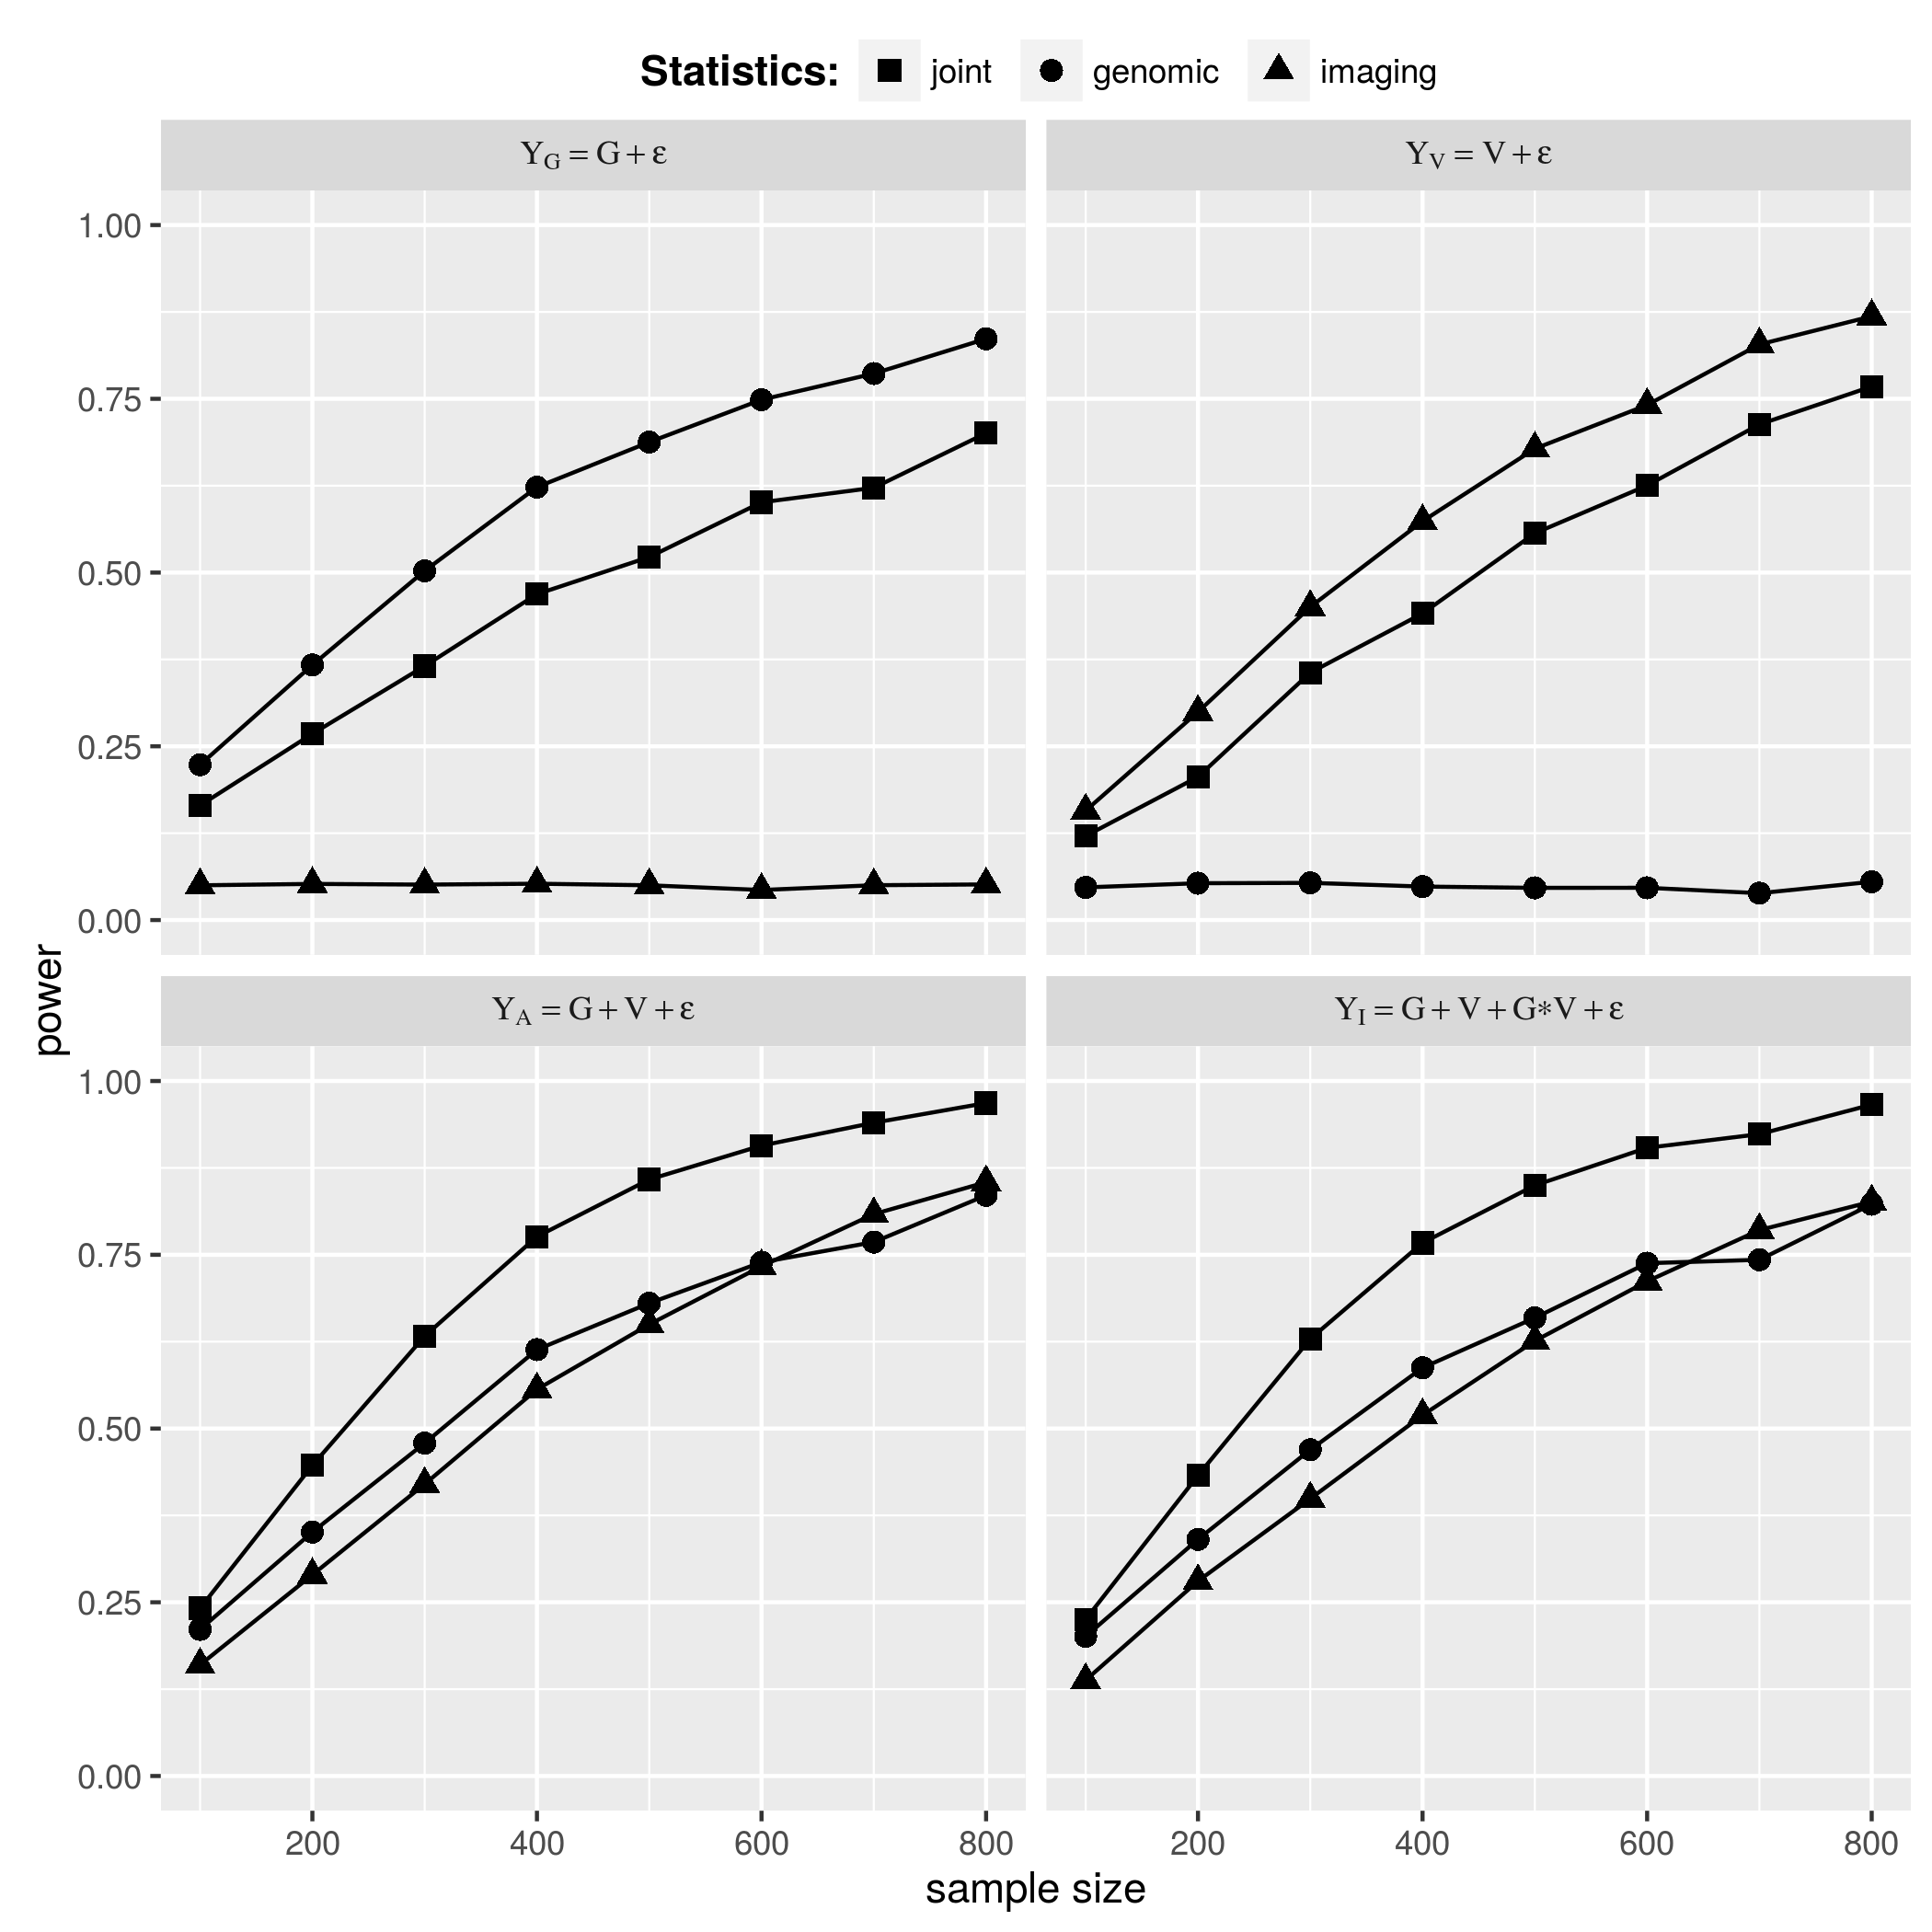
\includegraphics[width=300px]{img/PWR_CNT_KNL.png}
  \caption{Statistical power of the joint U-test versus genetic U-test and imaging U-test.}
  \label{fig:PWR_CNT_KNL}
\end{figure} 
%
\begin{figure}[!h]
  \centering
  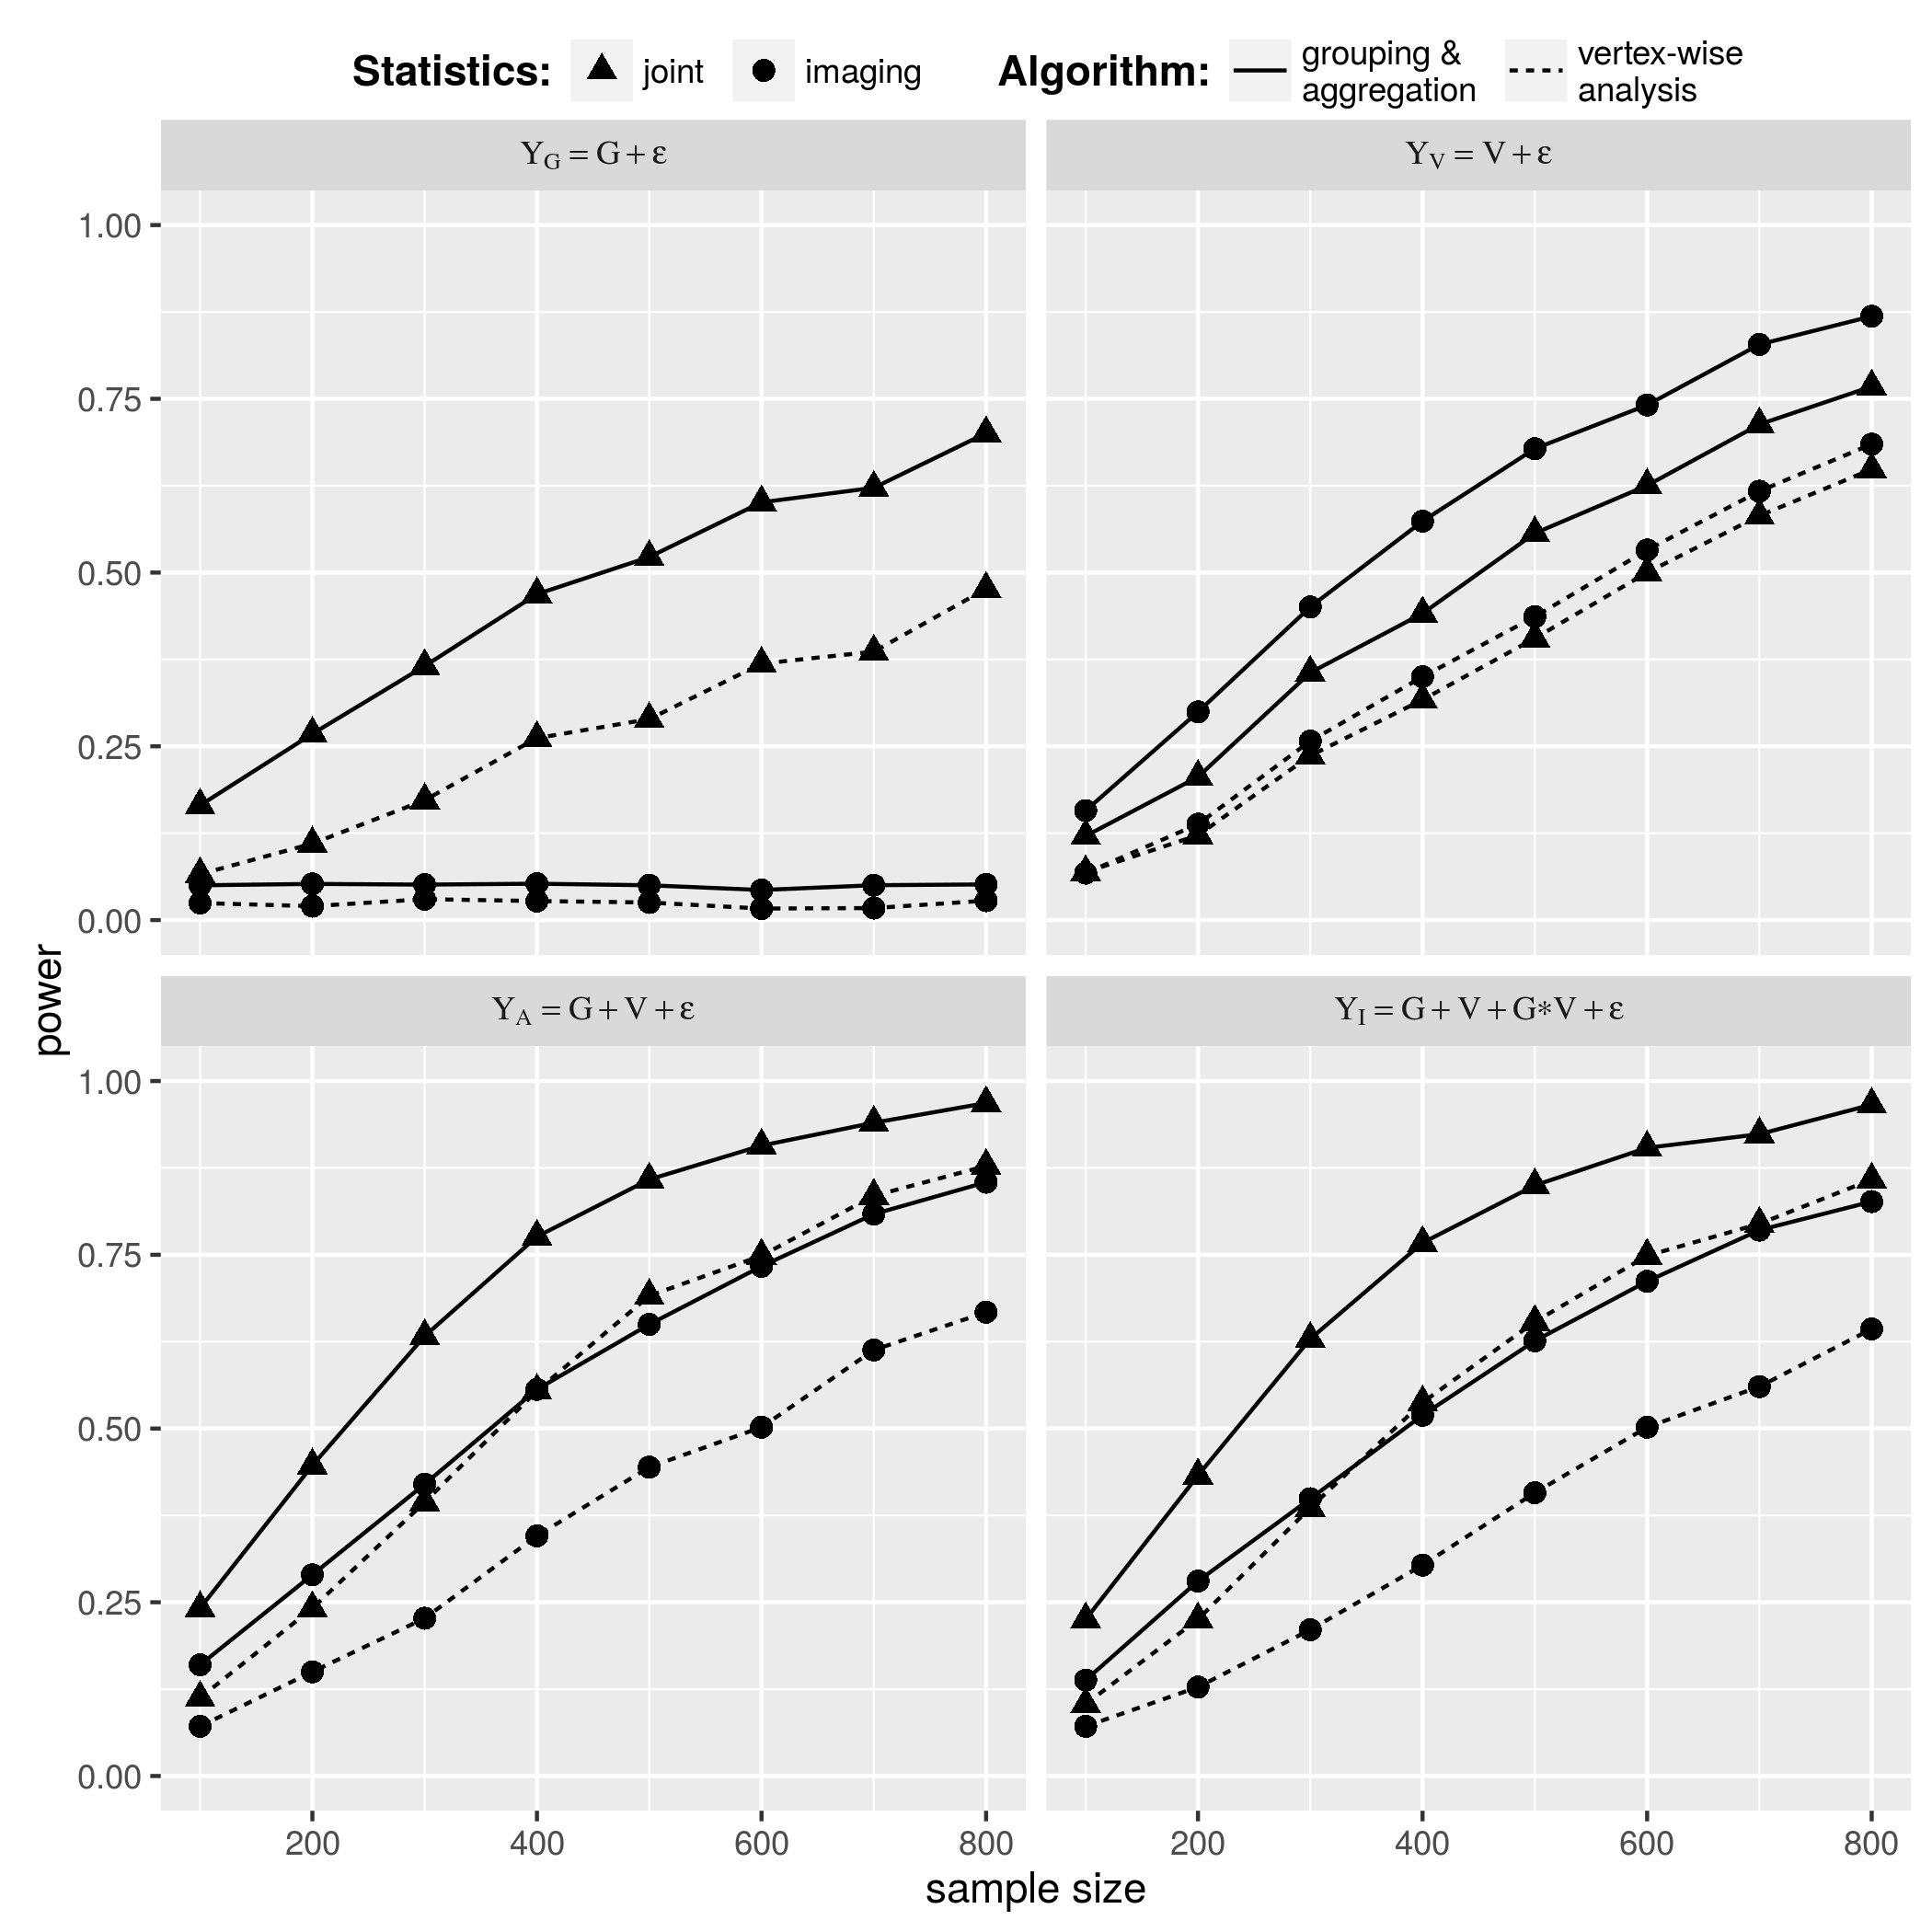
\includegraphics[width=300px]{img/PWR_CNT_VWA.png}
  \caption{Statistical power of the joint U-test and the imaging U-test with grouping versus vertex-wise analysis.}\label{fig:PWR_CNT_VWA}
\end{figure}
% 
\begin{figure}[!h]
  \centering
  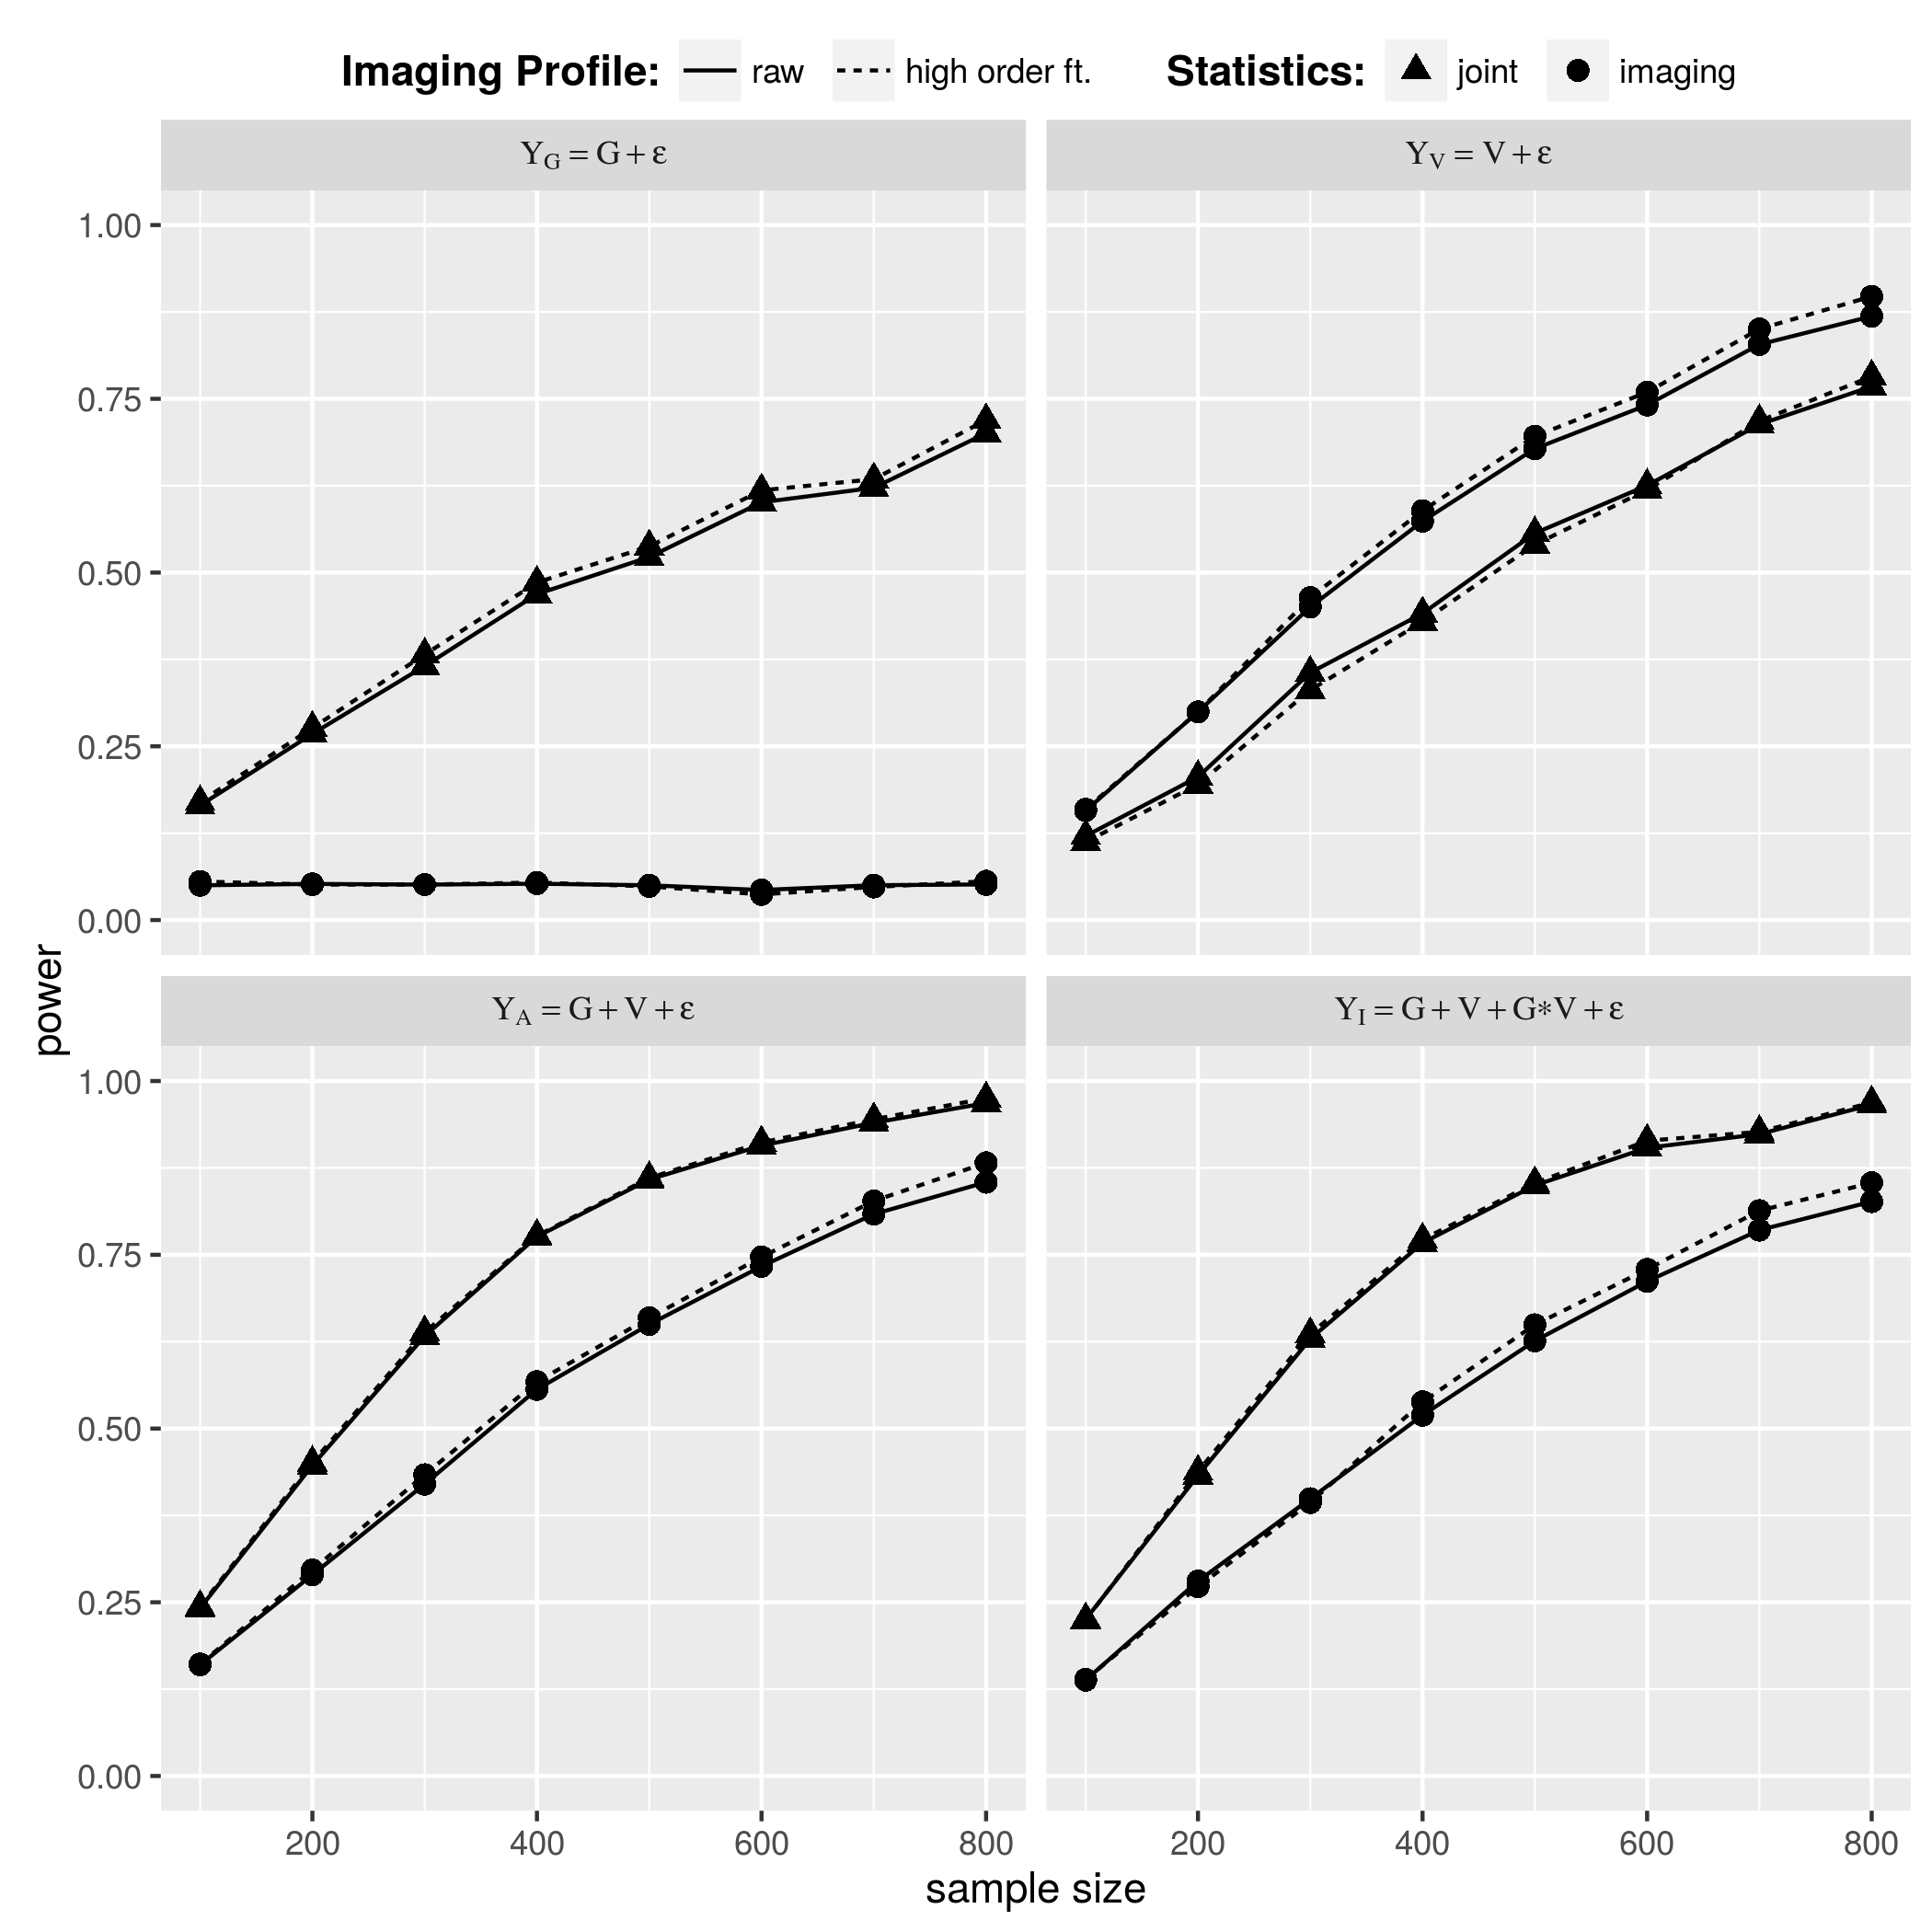
\includegraphics[width=300px]{img/PWR_CNT_SAE.png}
  \caption{Statistical power of the joint U-test and the imaging U-test with high order features versus original vertices.}\label{fig:PWR_CNT_SAE}
\end{figure}
% 
\begin{figure}[!h]
  \centering
  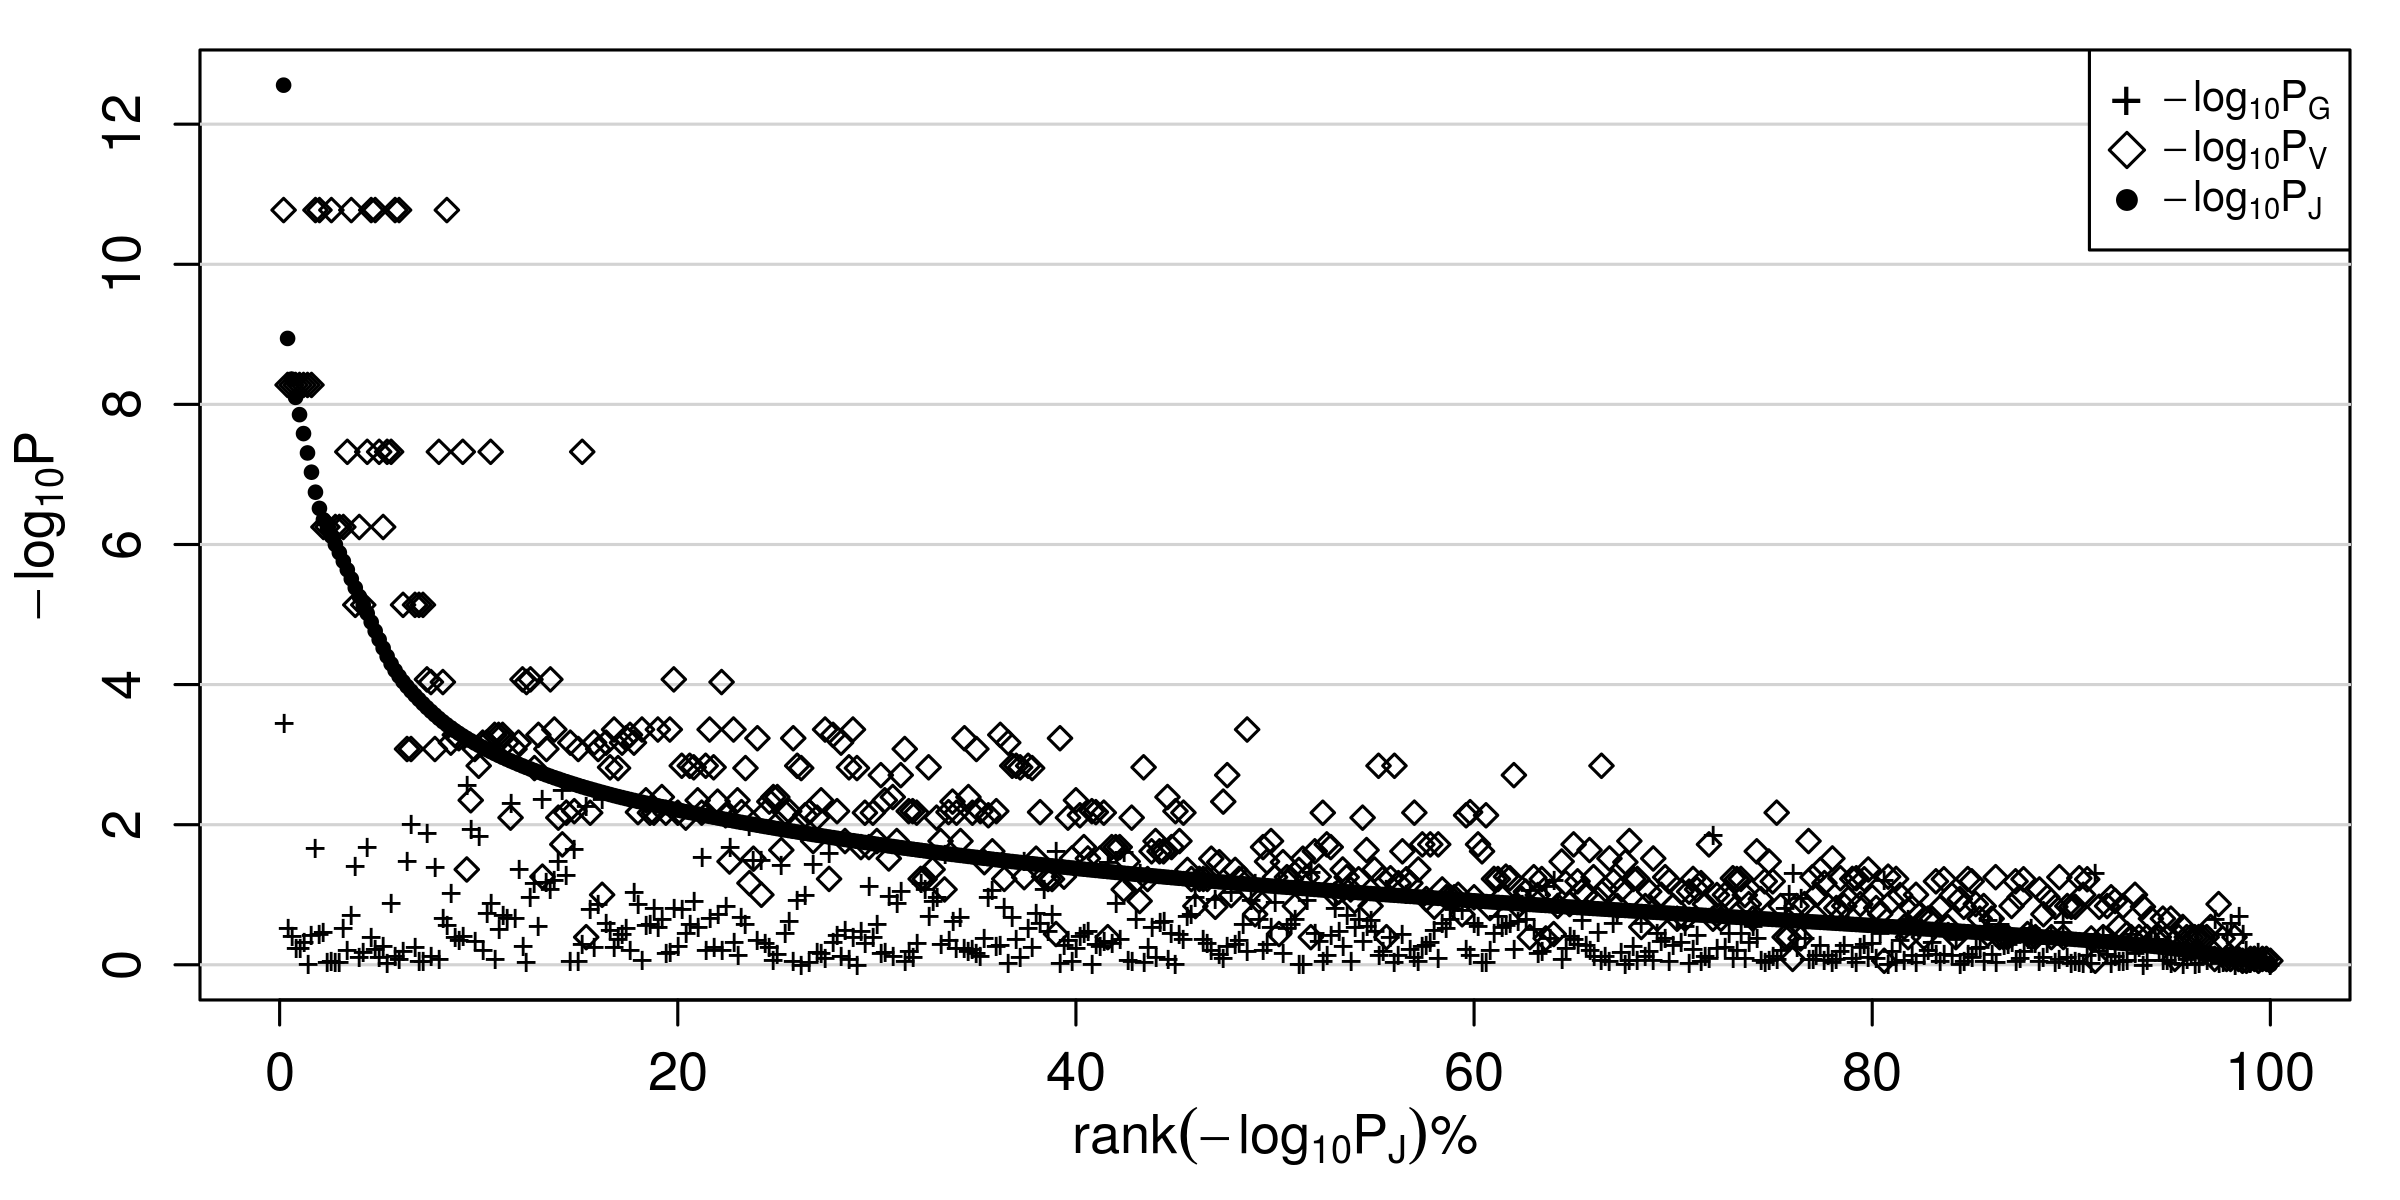
\includegraphics[width=300px]{img/RDA_PVL.png}
  \caption{Triplets of p-values $(P_J, P_G, P_V)$ for a joint test, gene-based only and imaging-based only from real data analysis.}\label{fig:RDA_PVL}
\end{figure}
\clearpage
\section*{Tables}
\begin{table}[!htbp]
  \centering
  \small
  \caption{Top 20 most significant joint test, overall}\label{tab:RDA_T20}
  % latex table generated in R 3.3.1 by xtable 1.8-0 package
% Fri Dec 23 17:55:43 2016
\begin{tabular}{llcclll}
  \hline
  GENE & CORTEX & $|V|$ & $|G|$ & $\qquad P_G$ & \qquad $P_V$ & \qquad $P_J$ \\ 
  \hline
  IGLV1-44 & l.superiortemporal & 7271 &  174 & $3.51 \times {10^{-04}}$ & $1.68 \times {10^{-11}}{_+^*}$ & $2.77 \times {10^{-13}}{_+^*}$ \\ 
  NBEAP2 & l.superiortemporal & 7271 &  238 & $1.19 \times {10^{-04}}$ & $1.68 \times {10^{-11}}{_+^*}$ & $4.74 \times {10^{-13}}{_+^*}$ \\ 
  RPL21P89 & l.superiortemporal & 7271 &   90 & $6.36 \times {10^{-04}}$ & $1.68 \times {10^{-11}}{_+^*}$ & $5.14 \times {10^{-13}}{_+^*}$ \\ 
  LOC102724504 & l.superiortemporal & 7271 &   59 & $1.41 \times {10^{-03}}$ & $1.68 \times {10^{-11}}{_+^*}$ & $5.56 \times {10^{-13}}{_+^*}$ \\ 
  CNTNAP3P8 & l.superiortemporal & 7271 &   40 & $1.08 \times {10^{-03}}$ & $1.68 \times {10^{-11}}{_+^*}$ & $6.17 \times {10^{-13}}{_+^*}$ \\ 
  CDH4 & l.superiortemporal & 7271 & 9464 & $4.64 \times {10^{-03}}$ & $1.68 \times {10^{-11}}{_+^*}$ & $6.96 \times {10^{-13}}{_+^*}$ \\ 
  HNRNPA1P19 & l.superiortemporal & 7271 &   17 & $8.88 \times {10^{-04}}$ & $1.68 \times {10^{-11}}{_+^*}$ & $7.80 \times {10^{-13}}{_+^*}$ \\ 
  FAM72C & l.superiortemporal & 7271 &  174 & $9.28 \times {10^{-06}}$ & $1.68 \times {10^{-11}}{_+^*}$ & $7.82 \times {10^{-13}}{_+^*}$ \\ 
  RP11-638L3.1 & l.superiortemporal & 7271 & 4067 & $1.41 \times {10^{-1}}$ & $1.68 \times {10^{-11}}{_+^*}$ & $9.49 \times {10^{-13}}{_+^*}$ \\ 
  CPXM1 & l.superiortemporal & 7271 &  208 & $8.78 \times {10^{-4}}$ & $1.68 \times {10^{-11}}{_+^*}$ & $1.08 \times {10^{-12}}{_+^*}$ \\ 
  LOC101929612 & l.superiortemporal & 7271 &  256 & $1.44 \times {10^{-2}}$ & $1.68 \times {10^{-11}}{_+^*}$ & $1.15 \times {10^{-12}}{_+^*}$ \\ 
  LOC100996517 & l.superiortemporal & 7271 &   34 & $6.77 \times {10^{-4}}$ & $1.68 \times {10^{-11}}{_+^*}$ & $1.20 \times {10^{-12}}{_+^*}$ \\ 
  IGLV5-45 & l.superiortemporal & 7271 &  179 & $3.44 \times {10^{-4}}$ & $1.68 \times {10^{-11}}{_+^*}$ & $1.23 \times {10^{-12}}{_+^*}$ \\ 
  MIS18BP1 & l.superiortemporal & 7271 &  553 & $4.95 \times {10^{-3}}$ & $1.68 \times {10^{-11}}{_+^*}$ & $1.35 \times {10^{-12}}{_+^*}$ \\ 
  CDR2 & l.superiortemporal & 7271 &  260 & $1.82 \times {10^{-4}}$ & $1.68 \times {10^{-11}}{_+^*}$ & $1.39 \times {10^{-12}}{_+^*}$ \\ 
  RPL41P2 & l.superiortemporal & 7271 &   87 & $6.04 \times {10^{-3}}$ & $1.68 \times {10^{-11}}{_+^*}$ & $1.59 \times {10^{-12}}{_+^*}$ \\ 
  LOC101927737 & l.superiortemporal & 7271 &  157 & $7.20 \times {10^{-3}}$ & $1.68 \times {10^{-11}}{_+^*}$ & $1.60 \times {10^{-12}}{_+^*}$ \\ 
  IGLV1-47 & l.superiortemporal & 7271 &  138 & $1.44 \times {10^{-2}}$ & $1.68 \times {10^{-11}}{_+^*}$ & $1.60 \times {10^{-12}}{_+^*}$ \\ 
  IGLV7-46 & l.superiortemporal & 7271 &  130 & $9.15 \times {10^{-4}}$ & $1.68 \times {10^{-11}}{_+^*}$ & $1.69 \times {10^{-12}}{_+^*}$ \\ 
  ZDHHC15 & l.superiortemporal & 7271 &   80 & $1.56 \times {10^{-3}}$ & $1.68 \times {10^{-11}}{_+^*}$ & $1.73 \times {10^{-12}}{_+^*}$ \\ 
  \hline
  \multicolumn{7}{l}{\texttt{*: below 0.05 after Bonferroni correction}} \\ 

  \multicolumn{7}{l}{\texttt{+: below 0.01 after FDR correction}}        \\ \hline
\end{tabular}

\end{table} 
% 
\begin{table}[!htbp]
  \centering
  \small
  \caption{top 20 most significant joint test, per cortex region}\label{tab:RDA_JNT}
  % latex table generated in R 3.3.1 by xtable 1.8-0 package
% Fri Dec 23 17:55:45 2016
\begin{tabular}{llcclll}
  \hline
GENE & CORTEX & $|V|$ & $|G|$ & $\qquad P_G$ & \qquad $P_V$ & \qquad $P_J$ \\ 
  \hline
IGLV1-44 & l.superiortemporal & 7271 &  174 & $3.51 \times {10^{-4}}$ & $1.68 \times {10^{-11}}{_+^*}$ & $2.77 \times {10^{-13}}{_+^*}$ \\ 
  ZNF749 & l.entorhinal & 1102 &  321 & $2.67 \times {10^{-5}}$ & $5.28 \times {10^{-9}}{_+^*}$ & $2.63 \times {10^{-11}}{_+^*}$ \\ 
  FAM72C & r.superiortemporal & 6868 &  174 & $9.28 \times {10^{-6}}$ & $4.75 \times {10^{-8}}{_+^*}$ & $2.14 \times {10^{-10}}{_+^*}$ \\ 
  ZNF749 & r.entorhinal &  902 &  321 & $2.67 \times {10^{-5}}$ & $5.62 \times {10^{-7}}{_+^*}$ & $1.08 \times {10^{-9}}{_+^*}$ \\ 
  FAM72C & l.cuneus & 1630 &  174 & $9.28 \times {10^{-6}}$ & $7.27 \times {10^{-6}}{_+^*}$ & $4.22 \times {10^{-9}}{_+^*}$ \\ 
  ZNF749 & l.fusiform & 4714 &  321 & $2.67 \times {10^{-5}}$ & $8.43 \times {10^{-5}}{_+^*}$ & $4.54 \times {10^{-8}}{_+}$ \\ 
  FAM72C & l.middletemporal & 4452 &  174 & $9.28 \times {10^{-6}}$ & $4.38 \times {10^{-4}}{_+^*}$ & $5.14 \times {10^{-8}}{_+}$ \\ 
  FAM72C & r.cuneus & 1638 &  174 & $9.28 \times {10^{-6}}$ & $8.31 \times {10^{-4}}{_+}$ & $6.33 \times {10^{-8}}{_+}$ \\ 
  ZNF749 & l.temporalpole &  839 &  321 & $2.67 \times {10^{-5}}$ & $9.20 \times {10^{-5}}{_+^*}$ & $7.05 \times {10^{-8}}{_+}$ \\ 
  FAM72C & r.precuneus & 7975 &  174 & $9.28 \times {10^{-6}}$ & $1.44 \times {10^{-3}}{_+}$ & $7.43 \times {10^{-8}}{_+}$ \\ 
  HSPD1P13 & l.pericalcarine & 1912 &   86 & $1.69 \times {10^{-5}}$ & $6.74 \times {10^{-4}}{_+^*}$ & $1.12 \times {10^{-7}}{_+}$ \\ 
  FAM72C & r.fusiform & 4661 &  174 & $9.28 \times {10^{-6}}$ & $5.83 \times {10^{-4}}{_+^*}$ & $1.18 \times {10^{-7}}{_+}$ \\ 
  HSPD1P13 & r.pericalcarine & 1823 &   86 & $1.69 \times {10^{-5}}$ & $5.22 \times {10^{-4}}{_+^*}$ & $1.50 \times {10^{-7}}{_+}$ \\ 
  FAM72C & r.precentral & 10705 &  174 & $9.28 \times {10^{-6}}$ & $6.73 \times {10^{-3}}$ & $2.15 \times {10^{-7}}{_+}$ \\ 
  HSPD1P13 & r.paracentral & 3831 &   86 & $1.69 \times {10^{-5}}$ & $1.91 \times {10^{-2}}$ & $2.41 \times {10^{-7}}{_+}$ \\ 
  ZNF749 & r.temporalpole &  817 &  321 & $2.67 \times {10^{-5}}$ & $1.55 \times {10^{-3}}{_+}$ & $3.30 \times {10^{-7}}{_+}$ \\ 
  FAM72C & l.precentral & 10740 &  174 & $9.28 \times {10^{-6}}$ & $6.62 \times {10^{-3}}$ & $3.94 \times {10^{-7}}{_+}$ \\ 
  FAM72C & l.superiorfrontal & 12179 &  174 & $9.28 \times {10^{-6}}$ & $1.96 \times {10^{-3}}{_+}$ & $4.39 \times {10^{-7}}{_+}$ \\ 
  FAM72C & l.postcentral & 9519 &  174 & $9.28 \times {10^{-6}}$ & $1.71 \times {10^{-2}}$ & $5.69 \times {10^{-7}}{_+}$ \\ 
  ZNF749 & l.insula & 5229 &  321 & $2.67 \times {10^{-5}}$ & $1.52 \times {10^{-3}}{_+}$ & $6.69 \times {10^{-7}}{_+}$ \\ 
   \hline
    \multicolumn{7}{l}{\texttt{*: below 0.05 after Bonferroni correction}} \\ 

    \multicolumn{7}{l}{\texttt{+: below 0.01 after FDR correction}}        \\ \hline
\end{tabular}

\end{table} 
%
\singlespacing
\bibliographystyle{\style}
\bibliography{ref}
% \printbibliography{}
%
\end{document}

%%% Local Variables:
%%% mode: latex
%%% TeX-master: t
%%% End:
\grid
